\documentclass{article}
\usepackage[utf8]{inputenc}

\title{Home assignment 3}
\author{Numerical Optimization and its Applications - Spring 2019\\Gil Ben Shalom, 301908877\\Tom Yaacov, 305578239}
\date{\today}

\usepackage[shortlabels]{enumitem}
\usepackage{pythontex}
\usepackage[most]{tcolorbox}
\usepackage{amsmath,amsthm,amssymb}
%\usepackage[dvipsnames]{xcolor}

\usepackage{fancyvrb}

\newcommand{\importandtypeset}[1]{
  \inputpygments{python}{py_files/#1.py}%
  \pyc{from py_files import #1}
}

\newcommand{\saveandshowplot}[1]{
  \begin{center}
  \includegraphics[width=0.85\textwidth]{#1}
  \end{center}
}

\newtheorem{lemma}{Lemma}

\AtBeginEnvironment{tcolorbox}{\scriptsize}

\begin{document}

\maketitle

\section{Equality constrained optimization}
\begin{enumerate}[(a)] 
\item The optimization problem that is given can be formulated to a single equality constrained optimization problem:
\[\max_{\mathbf{x}\in \mathbb{R}^3}x_1x_2+x_2x_3+x_1x_3 \quad s.t. \quad x_1+x_2+x_3-3=0\]
The Lagrangian of this method is
\[\mathcal{L}(\mathbf{x}, \lambda_1) =  x_1x_2+x_2x_3+x_1x_3 + \lambda_1(x_1+x_2+x_3-3) \]
and the solution of this problem is given by
\begin{align*}
\nabla \mathcal{L} = 0 &\Rightarrow 
\begin{cases}
x_2+x_3+\lambda_1 = 0\\
x_1+x_3+\lambda_1 = 0\\
x_1+x_2+\lambda_1 = 0 \\
x_1+x_2+x_3 = 0 \\
\end{cases}
&\Rightarrow \quad
\begin{cases}
x_1=1\\
x_2=1\\
x_3=1\\
\lambda_1=-2\\
\end{cases}
\end{align*}
\item In order to show that this critical point is a maximum point we'll first compute the Hessian of $\mathcal{L}$:
\[\nabla_{\mathbf{x}}^2 \mathcal{L}(\mathbf{x}, \lambda_1) = 
\begin{bmatrix} 
\frac{\partial^2 \mathcal{L}}{\partial x_1^2} & \frac{\partial ^2 \mathcal{L}}{\partial x_1\partial x_2} & \frac{\partial ^2 \mathcal{L}}{\partial x_1\partial x_3} \\
\frac{\partial^2 \mathcal{L}}{\partial x_2\partial x_1} & \frac{\partial ^2 \mathcal{L}}{\partial x_2^2} & \frac{\partial ^2 \mathcal{L}}{\partial x_2\partial x_3} \\
\frac{\partial^2 \mathcal{L}}{\partial x_3\partial x_1} & \frac{\partial ^2 \mathcal{L}}{\partial x_3\partial x_2} & \frac{\partial ^2 \mathcal{L}}{\partial x_3^2} 
\end{bmatrix}
 = 
 \begin{bmatrix} 
 0& 1 & 1 \\
  1& 0 & 1 \\
   1& 1 & 0 
 \end{bmatrix}
 \]
Next we'll show that the Hessian of the Lagrangian is negative
\[\mathbf{y}^T\nabla_{\mathbf{x}}^2\mathcal{L}\mathbf{y} <0 \quad \forall \mathbf{y}\in \mathbb{R}^3 \quad s.t. \quad \mathbf{y}^T\mathbf{1} = 0 , \mathbf{y}\ne \mathbf{0} \]
\begin{align*}
\mathbf{y}^T\nabla_{\mathbf{x}}^2\mathcal{L}\mathbf{y} &= 
 \begin{bmatrix} 
 y_1& y_2 & y_3 
 \end{bmatrix}
 \begin{bmatrix} 
  0& 1 & 1 \\
   1& 0 & 1 \\
    1& 1 & 0 
  \end{bmatrix}
   \begin{bmatrix} 
   y_1\\ y_2 \\ y_3 
   \end{bmatrix} \\ 
   &=
\begin{bmatrix} 
 y_2+y_3& y_1+y_3 & y_1+y_2 
 \end{bmatrix}
\begin{bmatrix} 
   y_1\\ y_2 \\ y_3 
   \end{bmatrix} 
\end{align*}
in addition,
\[\mathbf{y}^T\mathbf{1} = 0 \Rightarrow y_1+y_2+y_3 = 0 \Rightarrow 
\begin{bmatrix} 
 y_2+y_3\\ y_1+y_3 \\ y_1+y_2 
 \end{bmatrix}
 =
 \begin{bmatrix} 
    -y_1\\ -y_2 \\ -y_3 
    \end{bmatrix} 
\]
therefore, we get
\begin{align*}
\mathbf{y}^T\nabla_{\mathbf{x}}^2\mathcal{L}\mathbf{y}
&=
\begin{bmatrix}
 y_2+y_3& y_1+y_3 & y_1+y_2
 \end{bmatrix}
\begin{bmatrix}
   y_1\\ y_2 \\ y_3
   \end{bmatrix} \\
&=
\begin{bmatrix}
 -y_1& -y_2 & -y_3
 \end{bmatrix}
\begin{bmatrix}
   y_1\\ y_2 \\ y_3
   \end{bmatrix} \\
   &= -y_1^2 -y_2^2 -y_3^2 < 0 && *\mathbf{y}\ne \mathbf{0}
\end{align*}
\end{enumerate}
\section{General constrained optimization}
\begin{enumerate}[(a)]
\item The Lagrangian of this method is
\[
\mathcal{L}(\mathbf{x}, \lambda_1, \lambda_2, \lambda_3) =  (x_1 + x_2)^2 - 10(x_1 + x_2) + \lambda_1(3x_1  + x_2 - 6) + \lambda_2(x_1^2+x_2^2-5) + \lambda_3(-x_1)
\]
We will start by activating the first constraint and solve the equation. Meaning, we set $\lambda_2 = \lambda_3 = 0$
\begin{align*}
\nabla \mathcal{L} = 0 &\Rightarrow
\begin{cases}
2(x_1 + x_2) - 10 +3\lambda_1 = 0\\
2(x_1 + x_2) - 10 +\lambda_1 = 0\\
3x_1 + x_2 - 6 = 0 \\
\end{cases}
&\Rightarrow \quad
\begin{cases}
2x_1 + 2x_2 + 3\lambda_1 = 10\\
2x_1 + 2x_2 + \lambda_1 = 10 \\
3x_1 + x_2 = 6\\
\end{cases}
\end{align*}
The solution to this linear system is given by
\[x_1=\frac{1}{2}, x_2=\frac{9}{2}, \lambda_1=0\]
Using these values, we get that the second condition does not hold.
\[0.5^2 + 4.5^2 - 5 = 15 > 0 \]
Thus, we need to set the second constraint to be active as well. Thus, only $\lambda_3=0$. We get the following equations:
\begin{align*}
\nabla \mathcal{L} = 0 &\Rightarrow
\begin{cases}
2(x_1 + x_2) - 10 +3\lambda_1 + 2\lambda_2 x_1 = 0\\
2(x_1 + x_2) - 10 +\lambda_1 + 2\lambda_2 x_2 = 0\\
3x_1 + x_2 - 6 = 0 \\
x_1^2 + x_2^2 - 5 = 0
\end{cases}
&\Rightarrow \quad
\begin{cases}
2x_1 + 2x_2 + 3\lambda_1 + 2\lambda_2 x_1 = 10\\
2x_1 + 2x_2 + \lambda_1 + 2\lambda_2 x_2 = 10 \\
3x_1 + x_2 = 6\\
x_1^2 + x_2^2 = 5
\end{cases}
\end{align*}
The last two equations has 2 solution:
\[ x_1 = \frac{18-\sqrt{14}}{10},x_2 = \frac{3(2+\sqrt{14})}{10} \]
\[ x_1 = \frac{18+\sqrt{14}}{10},x_2 = -\frac{3(-2+\sqrt{14})}{10} \]
both of the solution holds for all the conditions, but the better solution for the minimization function is when $x_1 = \frac{18-\sqrt{14}}{10}=1.42,x_2 = \frac{3(2+\sqrt{14})}{10} = 1.72$, We will solve the first two equations to find $\lambda_1$ and $\lambda_2$:
\begin{align*}
\begin{cases}
2(x_1 + x_2) - 10 +3\lambda_1 + 2\lambda_2 x_1 = 0\\
2(x_1 + x_2) - 10 +\lambda_1 + 2\lambda_2 x_2 = 0
\end{cases}
&\Rightarrow \quad
\begin{cases}
3\lambda_1 + 2.85\lambda_2 = 3.72\\
\lambda_1 + 3.44\lambda_2 = 3.72
\end{cases}
\end{align*}
The solution is $\lambda_1=0.293,\lambda_2=1$
We will validate that all the KKT condition holds:
\[
\nabla \mathcal{L}(x^*, \lambda^{eq^{*}}, \lambda^{ieq^{*}}) =
\begin{bmatrix}
2*1.42 + 2*1.72 - 10 \\
2*1.42 + 2*1.72 - 10
\end{bmatrix}
+ 0.293
\begin{bmatrix}
3 \\
1
\end{bmatrix}
+ 1
\begin{bmatrix}
2*1.42 \\
2*1.72
\end{bmatrix}
= 0
\]

\[c^{eq}(x^*) = 0:\]
\[
3x_1 + x_2 - 6 = 3 * 1.42 + 1.72 - 6 = 0
\]

Second constraint is active, and the third not, and indeed $\lambda_2 > 0, \lambda_3 = 0.$

From all the above we can conclude that the KKT condition hold.
\item
\[
f_\mu(x) = (x_1 + x_2)^2 - 10(x_1 + x_2) + \mu [(3x_1 + x_2 - 6)^2 + (max\{(x_1^2 + x_2^2 - 5), 0\})^2 + (max\{-x_1, 0\})^2]
\]
\item The code that runs the algorithm:
\begin{scriptsize}
\begin{tcolorbox}[%
    enhanced,
    breakable,
    frame hidden,
    overlay broken = {
        \draw[line width=0.5mm, black, rounded corners]
        (frame.north west) rectangle (frame.south east);},
    ]{}
\inputpygments{python}{py_files/part_2_c.py}%
\end{tcolorbox}
\end{scriptsize}
Function and constraint results for each value of $\mu$
\begin{scriptsize}
\begin{tcolorbox}[%
    enhanced,
    breakable,
    frame hidden,
    overlay broken = {
        \draw[line width=0.5mm, black, rounded corners]
        (frame.north west) rectangle (frame.south east);},
    ]{}
\begingroup
\obeylines
\input{py_files/part_2_c_results.txt}
\endgroup%
\end{tcolorbox}
\end{scriptsize}
\end{enumerate}
\section{Box-constrained optimization}
\begin{enumerate}[(a)]
\item The scalar box constrained minimization problem can be formulated to general constrained optimization problem:
\[\min_{x\in \mathbb{R}}\frac{1}{2}hx^2-gx\quad s.t. \quad
\begin{cases}
-x+a \le 0\\
x-b \le 0
\end{cases}
\]
The Lagrangian of this method is
\[\mathcal{L}(x, \lambda_1, \lambda_2) =  \frac{1}{2}hx^2-gx + \lambda_1(-x+a) + \lambda_2(x-b)\]
We'll compute the first order necessary conditions: Suppose that $x^*$ is a local solution of the problem, than the following conditions hold:
\begin{enumerate}[(1)]
\item $\nabla_x\mathcal{L}(x^*, \lambda_1^*, \lambda_2^*) = hx^*-g -\lambda_1^*+\lambda_2^* = 0$
\item $-x^*+a \le 0$
\item $x^*-b \le 0$
\item $\lambda_1^* \ge 0$
\item $\lambda_2^* \ge 0$
\item $\lambda_1^*(-x^*+a) = 0$
\item $\lambda_2^*(x^*-b) = 0$
\end{enumerate}
To know whether a stationary point is a minimum or a maximum we have the second order necessary conditions for general constrained minimization:
\[\nabla_x^2\mathcal{L}(x^*, \lambda_1^*, \lambda_2^*) = h > 0\]
therefore
\[y\nabla_x^2\mathcal{L}(x^*, \lambda_1^*, \lambda_2^*)y  = yhy> 0 \quad \forall y \ne 0\]
and the stationary point is a minimum.\\
We can divide our solution to 3 cases:
\begin{enumerate}
\item $a \le \frac{g}{h} \le b$:\\
Solution: $x^* =  \frac{g}{h}, \lambda_1^* = 0, \lambda_2^* = 0$
we'll check that the first order necessary conditions hold:
\begin{enumerate}[(1)]
\item $\nabla_x\mathcal{L}(x^*, \lambda_1^*, \lambda_2^*) = hx^*-g -\lambda_1^*+\lambda_2^*  = h\frac{g}{h}-g -0+0 = 0$
\item $-x^*+a  = -\frac{g}{h}+a \le 0$
\item $x^*-b  = \frac{g}{h}-b\le 0$
\item $\lambda_1^*  = 0\ge 0$
\item $\lambda_2^*  = 0\ge 0$
\item $\lambda_1^*(-x^*+a) =0(-\frac{g}{h}+a) = 0$
\item $\lambda_2^*(x^*-b) = 0(\frac{g}{h}-b) = 0$
\end{enumerate}
\item $a > \frac{g}{h} $:\\
Solution: $x^* =  a, \lambda_1^* = ha-g, \lambda_2^* = 0$
we'll check that the first order necessary conditions hold:
\begin{enumerate}[(1)]
\item $\nabla_x\mathcal{L}(x^*, \lambda_1^*, \lambda_2^*) = hx^*-g -\lambda_1^*+\lambda_2^*  = ha-g -(ha-g)+0 = 0$
\item $-x^*+a  = -a+a \le 0$
\item $x^*-b  = a-b\le 0$
\item $\lambda_1^*  = ha-g>h\frac{g}{h}-g = 0$
\item $\lambda_2^*  = 0\ge 0$
\item $\lambda_1^*(-x^*+a) =(ha-g)(-a+a) = 0$
\item $\lambda_2^*(x^*-b) = 0(a-b) = 0$
\end{enumerate}
\item $\frac{g}{h} > b$:\\
Solution: $x^* =  b, \lambda_1^* = 0, \lambda_2^* =-hb+g$
we'll check that the first order necessary conditions hold:
\begin{enumerate}[(1)]
\item $\nabla_x\mathcal{L}(x^*, \lambda_1^*, \lambda_2^*) = hx^*-g -\lambda_1^*+\lambda_2^*  = hb-g -0-hb+g= 0$
\item $-x^*+a  = -b+a \le 0$
\item $x^*-b  = b-b\le 0$
\item $\lambda_1^*  = 0\ge  0$
\item $\lambda_2^*  = -hb+g > -h\frac{g}{h}+g = 0$
\item $\lambda_1^*(-x^*+a) =0(-b+a) = 0$
\item $\lambda_2^*(x^*-b) = (-hb+g)(b-b) = 0$
\end{enumerate}
\end{enumerate}
\item Let the following problem
\[\min_{\mathbf{x}\in \mathbb{R}^n}\frac{1}{2}\mathbf{x}^TH \mathbf{x}-\mathbf{x}^T\mathbf{g} \quad s.t. \quad \mathbf{a}\le \mathbf{x}\le \mathbf{b} \]
Therefore, the minimization for each scalar $x_i$ is given by
\begin{small}
\begin{align*}
argmin_{x_i\in \mathbb{R}}\frac{1}{2}\mathbf{x}^TH \mathbf{x}-\mathbf{x}^T\mathbf{g}
&= argmin_{x_i\in \mathbb{R}}\frac{1}{2}\Big(\sum_i\sum_jx_ix_jh_{i,j}\Big)-\sum_ix_ig_i\\
&= argmin_{x_i\in \mathbb{R}}\frac{1}{2}x_i^2h_{i,i}+\frac{1}{2}\Big(\sum_{j\ne i}x_ix_jh_{i,j}+x_ix_jh_{j,i}\Big)-x_ig_i &&*\text{\tiny removing consants-$x_j, j\ne i$}\\
&= argmin_{x_i\in \mathbb{R}}\frac{1}{2}x_i^2h_{i,i}+\frac{1}{2}2\Big(\sum_{j\ne i}x_ix_jh_{i,j}\Big)-x_ig_i &&*\text{$H$ symmetric}\\
&= argmin_{x_i\in \mathbb{R}}\frac{1}{2}x_i^2h_{i,i}+\Big(\Big(\sum_{j\ne i}x_jh_{i,j}\Big)-g_i\Big)x_i
\end{align*}
\end{small}

In addition, given that the rest are known:
\[\mathbf{a}\le \mathbf{x}\le \mathbf{b} \Rightarrow a_i \le x_i \le b_i\]
therefore, we get  that the minimization for each scalar $x_i$ is given by
\[\min_{x_i\in \mathbb{R}}\frac{1}{2}x_i^2h_{i,i}+\Big(\Big(\sum_{i\ne j}x_jh_{i,j}\Big)-g_i\Big)x_i \quad s.t. \quad a_i \le x_i \le b_i\]
In order to show the expression for the update of projected coordinate descent, we need to define the projection operation with respect to some norm and then set
\[x_i^{(k+1)} = \Pi_\Omega (x_i^{(k)} -\alpha \nabla f(x_i^{(k)})) \]
We will choose the squared $l_2$ norm. The lagrangian is given by
\[\mathcal{L}(x_i, \lambda_1, \lambda_2) = \frac{1}{2}||x_i-y_i||_2^2+\lambda_1(-x+a)+\lambda_2(x-b)       \]
and its gradient is given by
\[  \nabla_{x_i} \mathcal{L}(x_i, \lambda_1, \lambda_2) = x_i-y_i -\lambda_1+\lambda_2     \]
The problem is separable, so if $a_i \le x_i \le b_i$, then we can set $x_i^* = y_i$ without breaking the constraint, and hence $\lambda_1^*=\lambda_2^*=0$, because the
constraints are inactive. If $y_i < a_i$, then the lower bound constraint is active and the upper bound is not. We set $x_i^* = a_i$ and
\[x_i^* - y_i-\lambda_1 = 0 \Rightarrow\lambda_1 = a_i-y_i > 0 \]
We get a positive Lagrange multiplier, which is what needs to be. If $y_i>b_i$, then the upper bound constraint is active and the lower bound is not. We set $x_i^* = b_i$ and
\[x_i^* - y_i+\lambda_2 = 0 \Rightarrow\lambda_2 = y_i-b_i > 0 \]
The gradient is defined by
\[(\nabla f (x^{(k)}))_{(i)} = h_{i,i}x_i+\sum_{j\ne i}  h_{i,j}x_j -g_i   \]
and the step
\[z_i =  x_i^{(k)}-\alpha (\nabla f (x^{(k)}))_{(i)}   \]
Overall, the projected steepest descent step is given by:
\[x_i^{(k+1)} =
\begin{cases}
a_i &\quad z_i <a_i\\
b_i &\quad z_i >b_i\\
z_i &\quad otherwise\\
\end{cases}
\]

\item Following is an implementation for projected coordinate descent algorithm:
\begin{scriptsize}
\begin{tcolorbox}[%
    enhanced,
    breakable,
    frame hidden,
    overlay broken = {
        \draw[line width=0.5mm, black, rounded corners]
        (frame.north west) rectangle (frame.south east);},
    ]{}
\importandtypeset{part_3_c}
\end{tcolorbox}
\end{scriptsize}

\item Running the implementation over the given parameters and outputing the results:
\begin{scriptsize}
\begin{tcolorbox}[%
    enhanced,
    breakable,
    frame hidden,
    overlay broken = {
        \draw[line width=0.5mm, black, rounded corners]
        (frame.north west) rectangle (frame.south east);},
    ]{}
\importandtypeset{part_3_d}
\end{tcolorbox}
\end{scriptsize}
\end{enumerate}
\section{Projected Gradient Descent for the LASSO regression}
\begin{enumerate}[(a)]
\item \begin{lemma} \label{a}
let $\mathbf{u}, \mathbf{v}$ be the vectors that minimizes the objective\\ $||A(\mathbf{u} - \mathbf{v}) - \mathbf{b}||_2^2 + \lambda(1^T(\mathbf{u} + \mathbf{v}))$ $\Rightarrow \mathbf{u}, \mathbf{v}$ are from the following form:\\
$\forall i$ if $v_i > 0 \Rightarrow u_i=0$, if $u_i > 0 \Rightarrow v_i = 0$, else $u_i = v_i = 0$
\end{lemma}
\begin{proof}
Assume, for the sake of contradiction that there exists $\mathbf{u}$,$\mathbf{v}$ that minimizes the objective $||A(\mathbf{u} - \mathbf{v}) - \mathbf{b}||_2^2 + \lambda(1^T(\mathbf{u} + \mathbf{v}))$, and $\exists$ i s.t $u_i > 0$ and $v_i > 0$. Let $x=min(u_i, v_i)$. By Setting $u_i'=u_i - x, v_i'=v_i - x$, we keep the value of $\mathbf{u}-\mathbf{v}$ the same, thus the expression  $||A(\mathbf{u} - \mathbf{v}) - \mathbf{b}||_2^2$ doesn't change as well. But we reduce the value of $\lambda(1^T(\mathbf{u} + \mathbf{v}))$ in $2x\lambda$, and this a contradiction to the minimization of $\mathbf{u}$ and $\mathbf{v}$.
\end{proof}

\begin{lemma} \label{b}
For $\mathbf{u}, \mathbf{v}$ in the form we saw in Lemma1 $\Rightarrow$ let $\mathbf{x} = \mathbf{u} - \mathbf{v}$, than $\lambda(1^T(\mathbf{u} + \mathbf{v})) = \lambda||\mathbf{x}||_1$
\end{lemma}
\begin{proof}
\[
\lambda||\mathbf{x}||_1 = \lambda\sum_{i=1}^{n}|x_i| = \lambda\sum_{i=1}^{n} max\{x_i, -x_i\} = \lambda\sum_{i=1}^{n}max\{u_i-v_i, v_i-u_i\}
\]
From Lemma 1 we can conclude that
\[
max\{u_i-v_i, v_i-u_i\} = max\{u_i, v_i\} = u_i + v_i
\]
Thus:
\[
\lambda\sum_{i=1}^{n} max\{u_i-v_i, v_i-u_i\} = \lambda\sum_{i=1}^{n} (u_i + v_i) = \lambda(1^T(\mathbf{u} + \mathbf{v}))
\]
\end{proof}
Now, we proof the claim based on the 2 lemmas.
$\\ \Rightarrow\\$
Let $\mathbf{x}$ be the vector the minimizes the objective $||A\mathbf{x} - \mathbf{b}||_2^2 + \lambda||\mathbf{x}||_1$. We define $\mathbf{u}, \mathbf{v}$ s.t $\mathbf{x} = \mathbf{u}-\mathbf{v}$. $\forall$ i if $x_i > 0 \Rightarrow u_i = x_i, v_i = 0$, if $x_i < 0 \Rightarrow v_i = x_i, u_i = 0$, else $u_i = v_i = 0.\\$
Claim: The chosen $\mathbf{u}, \mathbf{v}$ Minimizes $||A(\mathbf{u} - \mathbf{v}) - \mathbf{b}||_2^2 + \lambda(1^T(\mathbf{u} + \mathbf{v})).\\$ Proof: Assume for the sake of contradiction the there exists $\mathbf{u}', \mathbf{v}'$ s.t  $||A(\mathbf{u}' - \mathbf{v}') - \mathbf{b}||_2^2 + \lambda(1^T(\mathbf{u}' + \mathbf{v}')) < ||A(\mathbf{u} - \mathbf{v}) - \mathbf{b}||_2^2 + \lambda(1^T(\mathbf{u} + \mathbf{v}))$, than, from Lemma1 and Lemma2, that means we can define $\mathbf{x}'=\mathbf{u}'-\mathbf{v}'$ and get that $||A\mathbf{x}' - \mathbf{b}||_2^2 + \lambda||\mathbf{x}'||_1 = ||A(\mathbf{u}' - \mathbf{v}') - \mathbf{b}||_2^2 + \lambda(1^T(\mathbf{u}' + \mathbf{v}')) < ||A(\mathbf{u} - \mathbf{v}) - \mathbf{b}||_2^2 + \lambda(1^T(\mathbf{u} + \mathbf{v})) =  ||A\mathbf{x} - \mathbf{b}||_2^2 + \lambda||\mathbf{x}||_1$ in contradiction to the minimization of $||\mathbf{x}||_1$.
$\\ \Leftarrow\\$
let $\mathbf{u}, \mathbf{v}$ be the vectors that minimize the objective $||A(\mathbf{u} - \mathbf{v}) - \mathbf{b}||_2^2 + \lambda(1^T(\mathbf{u} + \mathbf{v})).$ let $\mathbf{x} = \mathbf{u} - \mathbf{v}.\\$ Claim: $\mathbf{x}$ minimizes the objective $||A\mathbf{x} - \mathbf{b}||_2^2 + \lambda||\mathbf{x}||_1.\\$
Proof: Assume for the sake of contradiction that there exists $\mathbf{x}'$ s.t
$||A\mathbf{x}' - \mathbf{b}||_2^2 + \lambda||\mathbf{x}'||_1 < ||A\mathbf{x} - \mathbf{b}||_2^2 + \lambda||\mathbf{x}||_1$, We can declare $\mathbf{u}', \mathbf{v}'$ as seen in previous proof and get that $||A(\mathbf{u}' - \mathbf{v}') - \mathbf{b}||_2^2 + \lambda(1^T(\mathbf{u}' + \mathbf{v}')) = ||A\mathbf{x}' - \mathbf{b}||_2^2 + \lambda||\mathbf{x}'||_1 < ||A\mathbf{x} - \mathbf{b}||_2^2 + \lambda||\mathbf{x}||_1 = ||A(\mathbf{u} - \mathbf{v}) - \mathbf{b}||_2^2 + \lambda(1^T(\mathbf{u} + \mathbf{v}))$ in contradiction to the minimization of $\mathbf{u}, \mathbf{v}.$

\item The code that solves the problem:
\begin{scriptsize}
\begin{tcolorbox}[%
    enhanced,
    breakable,
    frame hidden,
    overlay broken = {
        \draw[line width=0.5mm, black, rounded corners]
        (frame.north west) rectangle (frame.south east);},
    ]{}
\inputpygments{python}{py_files/part_4_b.py}%
\end{tcolorbox}
\end{scriptsize}
\item We will use the steepest decent algorithm by setting $A'=[A\text{ }-A], \mathbf{x} = [\mathbf{u}\text{ }\mathbf{v}]$. $\lambda=3$ leads to a solution with approximately 10\% non zero values. The code that run the simulation:
\begin{scriptsize}
\begin{tcolorbox}[%
    enhanced,
    breakable,
    frame hidden,
    overlay broken = {
        \draw[line width=0.5mm, black, rounded corners]
        (frame.north west) rectangle (frame.south east);},
    ]{}
\inputpygments{python}{py_files/part_4_c.py}%
\end{tcolorbox}
\end{scriptsize}
 The distance of x from the algorithm, from the original x and number of non-zero values for each lambda:
\begin{scriptsize}
\begin{tcolorbox}[%
    enhanced,
    breakable,
    frame hidden,
    overlay broken = {
        \draw[line width=0.5mm, black, rounded corners]
        (frame.north west) rectangle (frame.south east);},
    ]{}
\begingroup
\obeylines
\input{py_files/4c_results.txt}
\endgroup%

\end{tcolorbox}
\end{scriptsize}
The objective value of each iteration, for each lambda:
\begin{scriptsize}
\begin{tcolorbox}[%
    enhanced,
    breakable,
    frame hidden,
    overlay broken = {
        \draw[line width=0.5mm, black, rounded corners]
        (frame.north west) rectangle (frame.south east);},
    ]{}
\begin{center}
  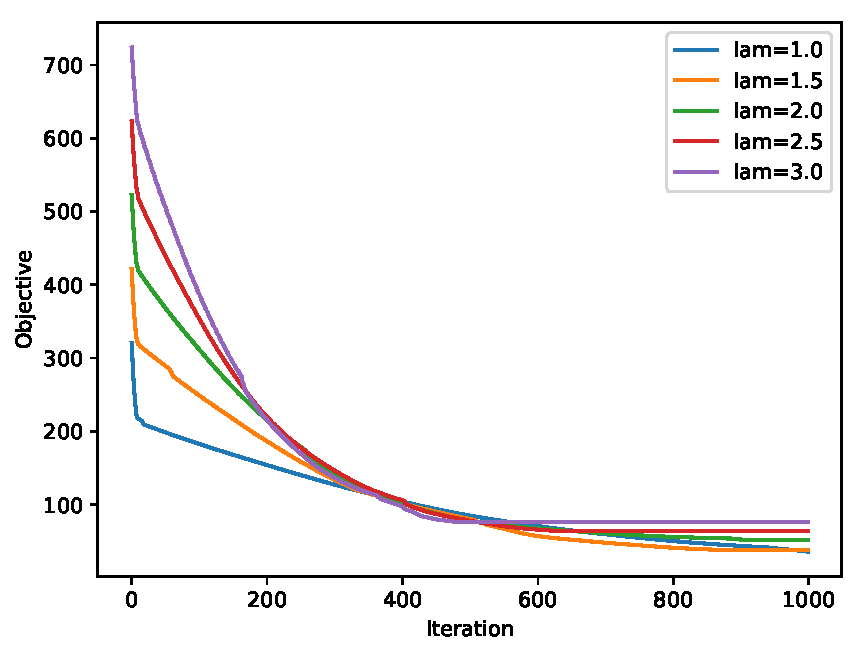
\includegraphics[width=0.85\textwidth]{py_files/4c_objectives}
\end{center}
\end{tcolorbox}
\end{scriptsize}
\item (non-mandatory)
\item (non-mandatory)
\end{enumerate}
\end{document}
